\chapter{Appendix}
\chaptermark{Appendix} 

% \textit{All work carried out by the SeniorStudent which is not part of the previous chapters, should be added to this Appendix. In the working folder each SeniorStudent stores the source files (such as PowerPoint (.pptx) Markdown (.md) files)
%  being part of the appendix in the subfolder ``7.Appendix''. The naming convention is: <appendix-prefix>.<title\_of\_the\_appendix>.}

% \textit{UMLet files which are part of the appendix are stored in the subfolder ``6.UMLet\_Sources`` using the following naming convention: ``<appendix-prefix>.<title\_of\_the\_contribution\_page>``. The UMLet diagram from the page ``MuleSoft System Environment at KIT`` of the appendix \ref{app:mul_sys_env_at_kit} can be taken as example.
% }

% \clearpage

% \renewcommand{\thesection}{\Alph{section}}
% \centering

% \section{WASA Contributions}
% \subsection{MuleSoft System Environment at KIT}
% \label{app:mul_sys_env_at_kit}

% % This command is used for the first or only one PDF page.
% 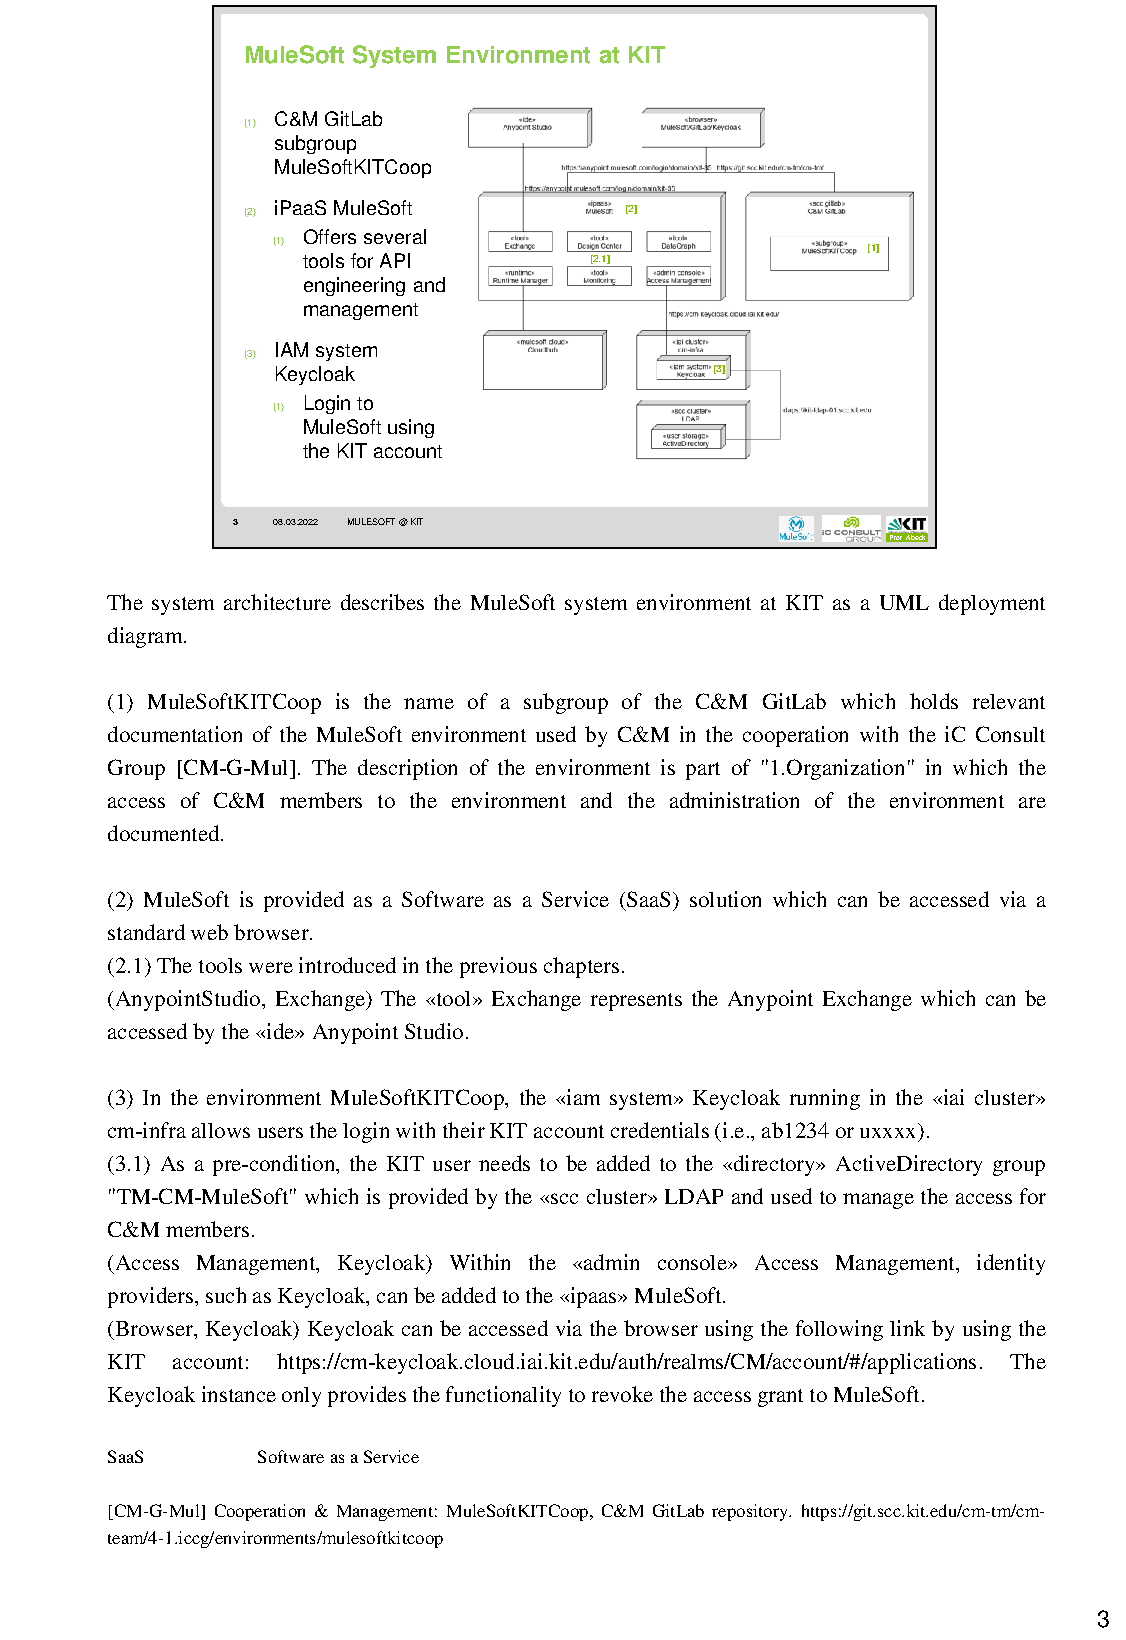
\includegraphics[height=0.9\textheight]{pdfs/a1.mulesoft_environment.pdf}

% % If more than one PDF page is included, the following command adds the additional PDF pages..
% \includepdf[pagecommand={\thispagestyle{plain}}, pages={2-last},height=0.9\textheight]{pdfs/a1.mulesoft_environment.pdf}
% \subsection{Next WASA Contribution ...}

% \clearpage
% \section{Best Practices}

% \subsection{Best Practices Template}
% 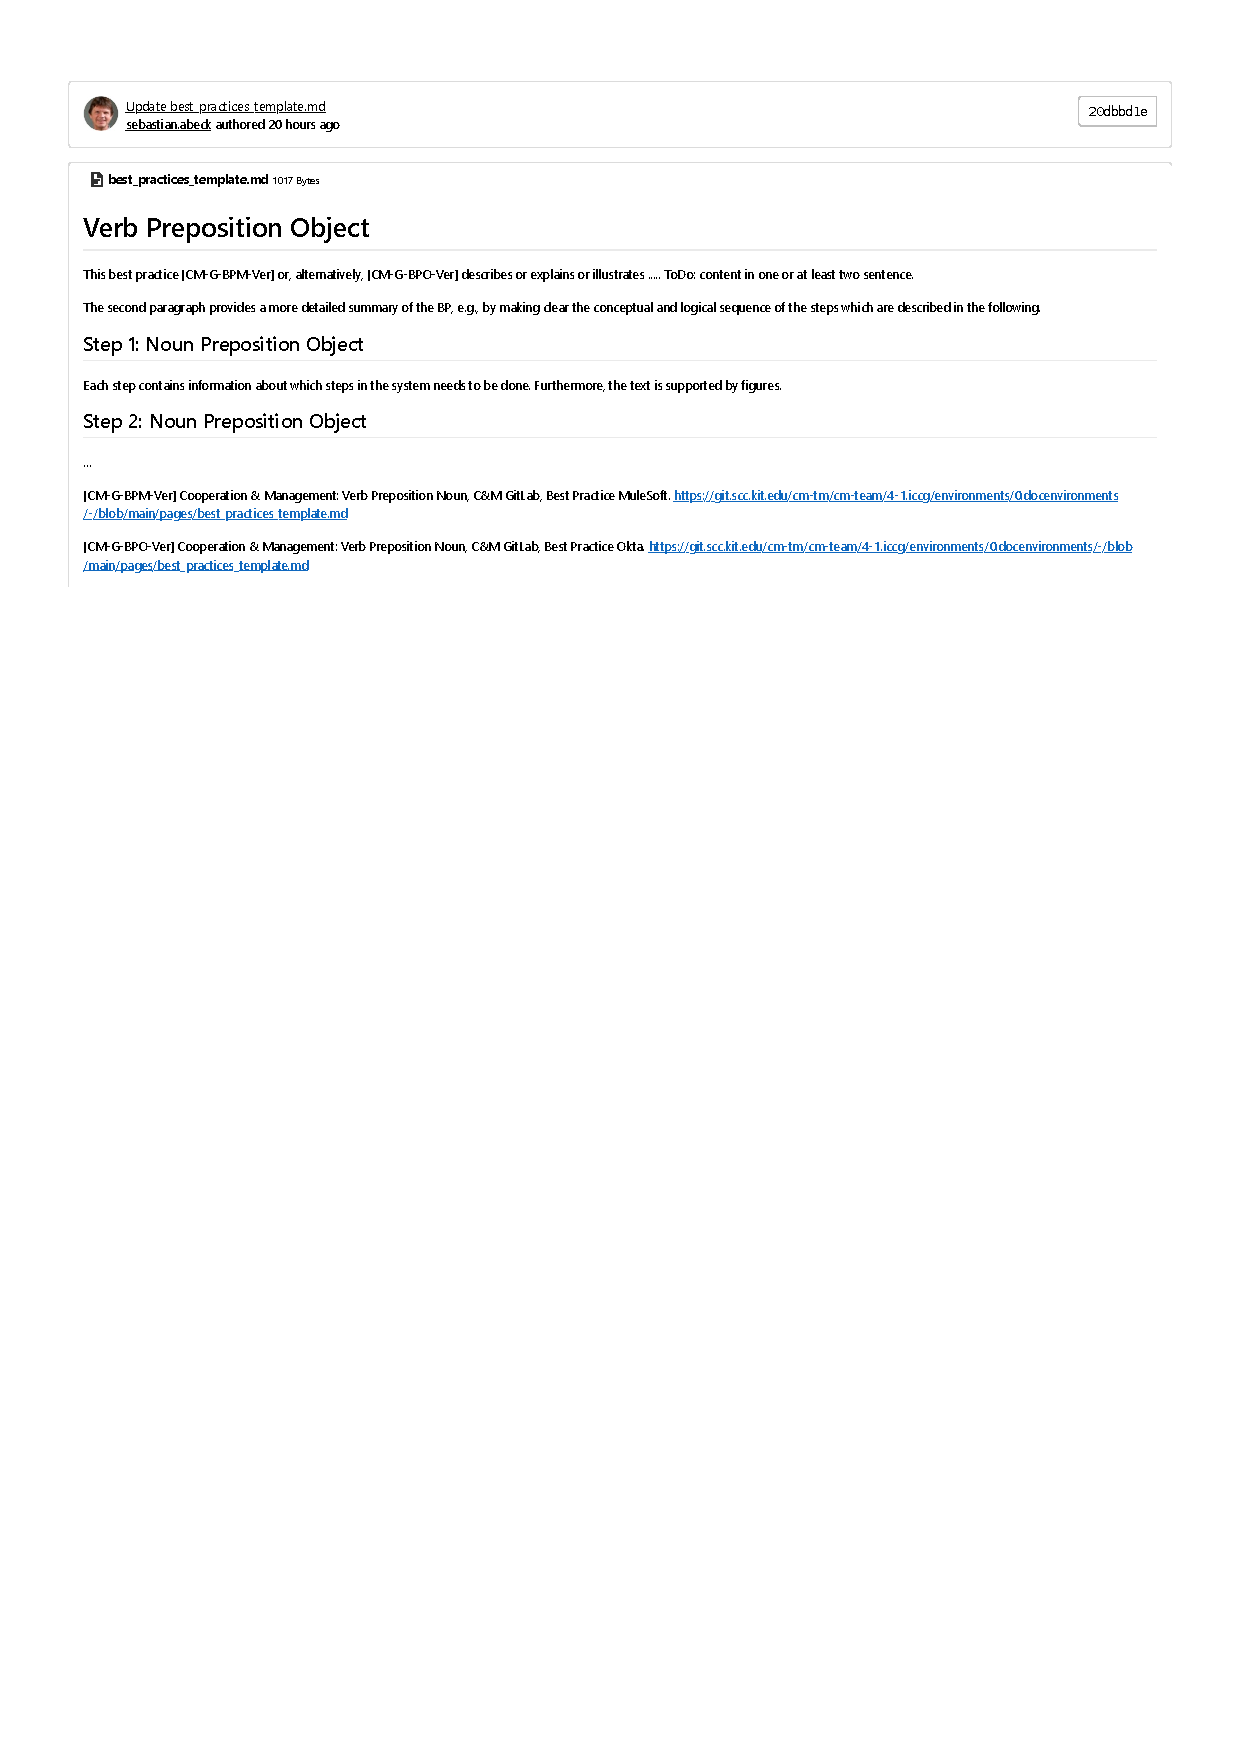
\includegraphics[height=0.9\textheight]{pdfs/b1.best_practice_template.pdf}

% \clearpage
% \section{Lunch and Learn}

% \clearpage
% \section{Miscellaneous}

% \clearpage
% \section{Publication Contributions}


\clearpage


%
% Bibliography
%
\makeatletter
\renewenvironment{thebibliography}[1]
     {\section{\bibname}
      \list{\@biblabel{\@arabic\c@enumiv}}
           {\settowidth\labelwidth{\@biblabel{#1}}
            \leftmargin\labelwidth
            \advance\leftmargin\labelsep
            \@openbib@code
            \usecounter{enumiv}%
            \let\p@enumiv\@empty
            \renewcommand\theenumiv{\@arabic\c@enumiv}}
      \sloppy
      \clubpenalty4000
      \@clubpenalty \clubpenalty
      \widowpenalty4000
      \sfcode`\.\@m}
     {\def\@noitemerr
       {\@latex@warning{Empty `thebibliography' environment}}%
      \endlist}
\makeatother

\bibliography{bt_engbrocks}

\bibliographystyle{cmnat}

%
% Insert PDFS
%
%\includepdf[pages=1, pagecommand={\section{Abschnitt} \thispagestyle{scrheadings}}, scale=0.7]{pdfs/anhang.pdf}
%\includepdf[pages=2-last, pagecommand={\thispagestyle{scrheadings}}, scale=0.7]{pdfs/anhang.pdf}